\documentclass{book}
\usepackage[a4paper,top=2.5cm,bottom=2.5cm,left=2.5cm,right=2.5cm]{geometry}
\usepackage{makeidx}
\usepackage{natbib}
\usepackage{graphicx}
\usepackage{multicol}
\usepackage{float}
\usepackage{listings}
\usepackage{color}
\usepackage{ifthen}
\usepackage[table]{xcolor}
\usepackage{textcomp}
\usepackage{alltt}
\usepackage{ifpdf}
\ifpdf
\usepackage[pdftex,
            pagebackref=true,
            colorlinks=true,
            linkcolor=blue,
            unicode
           ]{hyperref}
\else
\usepackage[ps2pdf,
            pagebackref=true,
            colorlinks=true,
            linkcolor=blue,
            unicode
           ]{hyperref}
\usepackage{pspicture}
\fi
\usepackage[utf8]{inputenc}
\usepackage[french]{babel}

\usepackage{mathptmx}
\usepackage[scaled=.90]{helvet}
\usepackage{courier}
\usepackage{sectsty}
\usepackage{amssymb}
\usepackage[titles]{tocloft}
\usepackage{doxygen}
\lstset{language=C++,inputencoding=utf8,basicstyle=\footnotesize,breaklines=true,breakatwhitespace=true,tabsize=8,numbers=left }
\makeindex
\setcounter{tocdepth}{3}
\renewcommand{\footrulewidth}{0.4pt}
\renewcommand{\familydefault}{\sfdefault}
\hfuzz=15pt
\setlength{\emergencystretch}{15pt}
\hbadness=750
\tolerance=750
\begin{document}
\hypersetup{pageanchor=false,citecolor=blue}
\begin{titlepage}
\vspace*{7cm}
\begin{center}
{\Large C\-R\-A\-B\-Ouest }\\
\vspace*{1cm}
{\large Généré par Doxygen 1.8.1.2}\\
\vspace*{0.5cm}
{\small Jeudi Octobre 8 2015 11:35:25}\\
\end{center}
\end{titlepage}
\clearemptydoublepage
\pagenumbering{roman}
\tableofcontents
\clearemptydoublepage
\pagenumbering{arabic}
\hypersetup{pageanchor=true,citecolor=blue}
\chapter{Liste des bogues}
\label{bug}
\hypertarget{bug}{}

\begin{DoxyRefList}
\item[\label{bug__bug000001}%
\hypertarget{bug__bug000001}{}%
Fichier \hyperlink{connexion_8cpp}{connexion.cpp} ]ne permet pas vraiment de s'inscrire, seulement de se connecter identifiant \-: afontraille mdp \-: 123 
\end{DoxyRefList}
\chapter{Index des espaces de nommage}
\section{Liste des espaces de nommage}
Liste de tous les espaces de nommage avec une brève description\-:\begin{DoxyCompactList}
\item\contentsline{section}{\hyperlink{namespace_ui}{Ui} }{\pageref{namespace_ui}}{}
\end{DoxyCompactList}

\chapter{Index des classes}
\section{Liste des classes}
Liste des classes, structures, unions et interfaces avec une brève description \-:\begin{DoxyCompactList}
\item\contentsline{section}{\hyperlink{classconnexion}{connexion} \\*Avec la classe connexion on retrouve des slots privés et publics ils permettent de valider ou tout simplement de fermer la fenêtre nous pouvons aussi gérer la couleur }{\pageref{classconnexion}}{}
\item\contentsline{section}{\hyperlink{classgestion}{gestion} \\*Avec la classe gestion on retrouve les slots privés ou public afin de gérer les différents rayons et produits on peut donc supprimer, ajouter ou modifier puis tout simplement les voir on peut également gérer la couleur }{\pageref{classgestion}}{}
\item\contentsline{section}{\hyperlink{class_main_window}{Main\-Window} \\*On peut retrouver des slots privés et publics qui permettent de quitter le programme et de se connecter }{\pageref{class_main_window}}{}
\end{DoxyCompactList}

\chapter{Index des fichiers}
\section{Liste des fichiers}
Liste de tous les fichiers avec une brève description \-:\begin{DoxyCompactList}
\item\contentsline{section}{/home/afontraille/\-Q\-T C\-R\-E\-A\-T\-O\-R/back\-Office\-N\-W/\hyperlink{connexion_8cpp}{connexion.\-cpp} \\*Permet de pouvoir se connecter ou s'inscrire dans New World }{\pageref{connexion_8cpp}}{}
\item\contentsline{section}{/home/afontraille/\-Q\-T C\-R\-E\-A\-T\-O\-R/back\-Office\-N\-W/\hyperlink{connexion_8h}{connexion.\-h} \\*Permet de pouvoir se connecter ou s'inscrire dans New World }{\pageref{connexion_8h}}{}
\item\contentsline{section}{/home/afontraille/\-Q\-T C\-R\-E\-A\-T\-O\-R/back\-Office\-N\-W/\hyperlink{gestion_8cpp}{gestion.\-cpp} \\*Permet de pouvoir gérer les produits et les rayons }{\pageref{gestion_8cpp}}{}
\item\contentsline{section}{/home/afontraille/\-Q\-T C\-R\-E\-A\-T\-O\-R/back\-Office\-N\-W/\hyperlink{gestion_8h}{gestion.\-h} \\*Permet de pouvoir gérer les produits et les rayons }{\pageref{gestion_8h}}{}
\item\contentsline{section}{/home/afontraille/\-Q\-T C\-R\-E\-A\-T\-O\-R/back\-Office\-N\-W/\hyperlink{main_8cpp}{main.\-cpp} \\*Main est obligatoire dans tout les programmes c++ }{\pageref{main_8cpp}}{}
\item\contentsline{section}{/home/afontraille/\-Q\-T C\-R\-E\-A\-T\-O\-R/back\-Office\-N\-W/\hyperlink{mainwindow_8cpp}{mainwindow.\-cpp} }{\pageref{mainwindow_8cpp}}{}
\item\contentsline{section}{/home/afontraille/\-Q\-T C\-R\-E\-A\-T\-O\-R/back\-Office\-N\-W/\hyperlink{mainwindow_8h}{mainwindow.\-h} }{\pageref{mainwindow_8h}}{}
\end{DoxyCompactList}

\chapter{Documentation des espaces de nommage}
\hypertarget{namespace_ui}{\section{Référence de l'espace de nommage Ui}
\label{namespace_ui}\index{Ui@{Ui}}
}

\chapter{Documentation des classes}
\hypertarget{classconnexion}{\section{Référence de la classe connexion}
\label{classconnexion}\index{connexion@{connexion}}
}


avec la classe connexion on retrouve des slots privés et publics ils permettent de valider ou tout simplement de fermer la fenêtre nous pouvons aussi gérer la couleur  




{\ttfamily \#include $<$connexion.\-h$>$}



Graphe de collaboration de connexion\-:\nopagebreak
\begin{figure}[H]
\begin{center}
\leavevmode
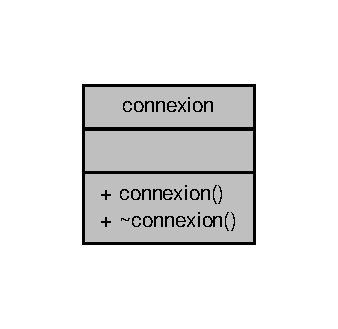
\includegraphics[width=162pt]{classconnexion__coll__graph}
\end{center}
\end{figure}
\subsection*{Fonctions membres publiques}
\begin{DoxyCompactItemize}
\item 
\hyperlink{classconnexion_a9764293a65b53a8385b6cc1d2ea14746}{connexion} (Q\-Widget $\ast$parent=0)
\begin{DoxyCompactList}\small\item\em permet de pouvoir se connecter à la base de données Si l'identifiant de la base de données ou le mdp est incorrect Alors il sera impossible de se connecter et un message d'erreur apparaitra \end{DoxyCompactList}\item 
\hyperlink{classconnexion_a28451b226398ff815107aa8a0fe4c673}{$\sim$connexion} ()
\begin{DoxyCompactList}\small\item\em \hyperlink{classconnexion_a28451b226398ff815107aa8a0fe4c673}{connexion\-::$\sim$connexion} \end{DoxyCompactList}\end{DoxyCompactItemize}


\subsection{Description détaillée}
avec la classe connexion on retrouve des slots privés et publics ils permettent de valider ou tout simplement de fermer la fenêtre nous pouvons aussi gérer la couleur 

Définition à la ligne 27 du fichier connexion.\-h.



\subsection{Documentation des constructeurs et destructeur}
\hypertarget{classconnexion_a9764293a65b53a8385b6cc1d2ea14746}{\index{connexion@{connexion}!connexion@{connexion}}
\index{connexion@{connexion}!connexion@{connexion}}
\subsubsection[{connexion}]{\setlength{\rightskip}{0pt plus 5cm}connexion\-::connexion (
\begin{DoxyParamCaption}
\item[{Q\-Widget $\ast$}]{parent = {\ttfamily 0}}
\end{DoxyParamCaption}
)\hspace{0.3cm}{\ttfamily [explicit]}}}\label{classconnexion_a9764293a65b53a8385b6cc1d2ea14746}


permet de pouvoir se connecter à la base de données Si l'identifiant de la base de données ou le mdp est incorrect Alors il sera impossible de se connecter et un message d'erreur apparaitra 


\begin{DoxyParams}{Paramètres}
{\em parent} & \\
\hline
\end{DoxyParams}


Définition à la ligne 26 du fichier connexion.\-cpp.


\begin{DoxyCode}
                                    :
    QDialog(parent),
    ui(\textcolor{keyword}{new} Ui::connexion)
\{
    ui->setupUi(\textcolor{keyword}{this});
    couleur();
    QSqlDatabase db=QSqlDatabase::addDatabase(\textcolor{stringliteral}{"QMYSQL"});
    maBase=\textcolor{keyword}{new} QSqlDatabase(db);
    maBase->setHostName(\textcolor{stringliteral}{"localhost"});
    maBase->setDatabaseName(\textcolor{stringliteral}{"testQT"});
    maBase->setUserName(\textcolor{stringliteral}{"afontraille"});
    maBase->setPassword(\textcolor{stringliteral}{"dTj124fs"});
    \textcolor{keywordtype}{bool} ok = maBase->open();
    \textcolor{keywordflow}{if}(!ok)
    \{
        QMessageBox::warning(\textcolor{keyword}{this},\textcolor{stringliteral}{"New World BackOffice"},\textcolor{stringliteral}{"La connexion à la
       base de données a échoué\(\backslash\)nVeuillez vérifier que le service mysql est lancé sur
       localhost"},QMessageBox::Ok|QMessageBox::Cancel,QMessageBox::Ok);
    \}
\}
\end{DoxyCode}
\hypertarget{classconnexion_a28451b226398ff815107aa8a0fe4c673}{\index{connexion@{connexion}!$\sim$connexion@{$\sim$connexion}}
\index{$\sim$connexion@{$\sim$connexion}!connexion@{connexion}}
\subsubsection[{$\sim$connexion}]{\setlength{\rightskip}{0pt plus 5cm}connexion\-::$\sim$connexion (
\begin{DoxyParamCaption}
{}
\end{DoxyParamCaption}
)}}\label{classconnexion_a28451b226398ff815107aa8a0fe4c673}


\hyperlink{classconnexion_a28451b226398ff815107aa8a0fe4c673}{connexion\-::$\sim$connexion} 



Définition à la ligne 48 du fichier connexion.\-cpp.


\begin{DoxyCode}
\{
    \textcolor{keyword}{delete} ui;
\}
\end{DoxyCode}


La documentation de cette classe a été générée à partir des fichiers suivants \-:\begin{DoxyCompactItemize}
\item 
/home/afontraille/\-Q\-T C\-R\-E\-A\-T\-O\-R/back\-Office\-N\-W/\hyperlink{connexion_8h}{connexion.\-h}\item 
/home/afontraille/\-Q\-T C\-R\-E\-A\-T\-O\-R/back\-Office\-N\-W/\hyperlink{connexion_8cpp}{connexion.\-cpp}\end{DoxyCompactItemize}

\hypertarget{classgestion}{\section{Référence de la classe gestion}
\label{classgestion}\index{gestion@{gestion}}
}


Avec la classe gestion on retrouve les slots privés ou public afin de gérer les différents rayons et produits on peut donc supprimer, ajouter ou modifier puis tout simplement les voir on peut également gérer la couleur.  




{\ttfamily \#include $<$gestion.\-h$>$}



Graphe de collaboration de gestion\-:\nopagebreak
\begin{figure}[H]
\begin{center}
\leavevmode
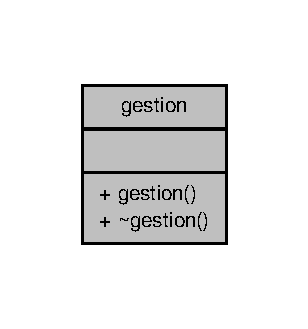
\includegraphics[width=148pt]{classgestion__coll__graph}
\end{center}
\end{figure}
\subsection*{Fonctions membres publiques}
\begin{DoxyCompactItemize}
\item 
\hyperlink{classgestion_a56a870ef0bef1cb98c679a1fa4bb25ff}{gestion} (Q\-Widget $\ast$parent=0)
\begin{DoxyCompactList}\small\item\em Si lorsque l'identifiant ou le mdp de la base de données est incorrect alors un msg d'erreur apparait sinon, la connexion a la base se fait bien, et ouvre alors la page connexion. \end{DoxyCompactList}\item 
\hyperlink{classgestion_a56c8770c7068cf05c9363b632f960838}{$\sim$gestion} ()
\end{DoxyCompactItemize}


\subsection{Description détaillée}
Avec la classe gestion on retrouve les slots privés ou public afin de gérer les différents rayons et produits on peut donc supprimer, ajouter ou modifier puis tout simplement les voir on peut également gérer la couleur. 

Définition à la ligne 32 du fichier gestion.\-h.



\subsection{Documentation des constructeurs et destructeur}
\hypertarget{classgestion_a56a870ef0bef1cb98c679a1fa4bb25ff}{\index{gestion@{gestion}!gestion@{gestion}}
\index{gestion@{gestion}!gestion@{gestion}}
\subsubsection[{gestion}]{\setlength{\rightskip}{0pt plus 5cm}gestion\-::gestion (
\begin{DoxyParamCaption}
\item[{Q\-Widget $\ast$}]{parent = {\ttfamily 0}}
\end{DoxyParamCaption}
)\hspace{0.3cm}{\ttfamily [explicit]}}}\label{classgestion_a56a870ef0bef1cb98c679a1fa4bb25ff}


Si lorsque l'identifiant ou le mdp de la base de données est incorrect alors un msg d'erreur apparait sinon, la connexion a la base se fait bien, et ouvre alors la page connexion. 


\begin{DoxyParams}{Paramètres}
{\em parent} & \\
\hline
\end{DoxyParams}


Définition à la ligne 26 du fichier gestion.\-cpp.


\begin{DoxyCode}
                                :
    QDialog(parent),
    ui(\textcolor{keyword}{new} Ui::gestion)
\{
    ui->setupUi(\textcolor{keyword}{this});
    couleur();
    QSqlDatabase db=QSqlDatabase::addDatabase(\textcolor{stringliteral}{"QMYSQL"});
    maBase=\textcolor{keyword}{new} QSqlDatabase(db);
    maBase->setHostName(\textcolor{stringliteral}{"localhost"});
    maBase->setDatabaseName(\textcolor{stringliteral}{"testQT"});
    maBase->setUserName(\textcolor{stringliteral}{"afontraille"});
    maBase->setPassword(\textcolor{stringliteral}{"dTj124fs"});
    \textcolor{keywordtype}{bool} ok = maBase->open();
    \textcolor{keywordflow}{if}(!ok)
    \{
        QMessageBox::warning(\textcolor{keyword}{this},\textcolor{stringliteral}{"New World BackOffice"},\textcolor{stringliteral}{"La connexion à la
       base de données a échoué \(\backslash\)n Veuillez vérifier que le service mysql est lancé sur
       localhost"},QMessageBox::Ok|QMessageBox::Cancel,QMessageBox::Ok);
    \}
    \textcolor{keywordflow}{else}
    \{
        modelRayon=\textcolor{keyword}{new} QSqlTableModel(\textcolor{keyword}{this},*maBase);
        modelRayon->setTable(\textcolor{stringliteral}{"surType"});
        ui->tableViewRayons->setModel(modelRayon);
        modelRayon->select();
        modelRayon->setHeaderData(1,Qt::Horizontal, trUtf8(\textcolor{stringliteral}{"Nom"}));
        modelRayon->setEditStrategy(QSqlTableModel::OnFieldChange);

        modelProduit=\textcolor{keyword}{new} QSqlRelationalTableModel(\textcolor{keyword}{this},*maBase);
        modelProduit->setTable(\textcolor{stringliteral}{"type"});
        ui->tableViewProduits->setModel(modelProduit);
        modelProduit->setRelation(2, QSqlRelation(\textcolor{stringliteral}{"surType"}, \textcolor{stringliteral}{"no"}, \textcolor{stringliteral}{"
      libelleSurType"}));
        modelProduit->select();
        modelProduit->setHeaderData(1,Qt::Horizontal, trUtf8(\textcolor{stringliteral}{"Nom"}));
        modelProduit->setHeaderData(2,Qt::Horizontal, trUtf8(\textcolor{stringliteral}{"Nom du rayon"}));

        \textcolor{comment}{//Cacher l'identifiant pour les rayons et les produits}
        ui->tableViewRayons->hideColumn(0);
        ui->tableViewProduits->hideColumn(0);
        modelProduit->setEditStrategy(QSqlRelationalTableModel::OnRowChange);

        \textcolor{comment}{//REMPLIR COMBO BOX AJOUT}
        QString requete=\textcolor{stringliteral}{"select * from surType;"};
        \textcolor{comment}{//exécution de la requête}
        QSqlQuery reqEx(requete);
        \textcolor{comment}{//compteur de lignes}
        \textcolor{keywordtype}{int} i=0;
        \textcolor{comment}{//boucle pour remplir ma comboBox}
        \textcolor{keywordflow}{while}(reqEx.next())
        \{
            ui->comboBox->addItem(reqEx.value(1).toString(), i);
            i++;
        \}
        \textcolor{comment}{//REMPLIR COMBO BOX MODIF}
        QString req=\textcolor{stringliteral}{"select * from surType;"};
        \textcolor{comment}{//exécution de la requête}
        QSqlQuery reqExModif(req);
        \textcolor{comment}{//compteur de lignes}
        \textcolor{keywordtype}{int} j=0;
        \textcolor{comment}{//boucle pour remplir ma comboBox}
        \textcolor{keywordflow}{while}(reqExModif.next())
        \{
            ui->comboBoxModif->addItem(reqExModif.value(1).toString(), j);
            i++;
        \}
        \textcolor{comment}{//Désactiver les boutons}
        \textcolor{comment}{/*if()}
\textcolor{comment}{        \{}
\textcolor{comment}{            ui->pushButtonAddProduit->setEnabled(false);}
\textcolor{comment}{        \}*/}
    \}
\}
\end{DoxyCode}
\hypertarget{classgestion_a56c8770c7068cf05c9363b632f960838}{\index{gestion@{gestion}!$\sim$gestion@{$\sim$gestion}}
\index{$\sim$gestion@{$\sim$gestion}!gestion@{gestion}}
\subsubsection[{$\sim$gestion}]{\setlength{\rightskip}{0pt plus 5cm}gestion\-::$\sim$gestion (
\begin{DoxyParamCaption}
{}
\end{DoxyParamCaption}
)}}\label{classgestion_a56c8770c7068cf05c9363b632f960838}


Définition à la ligne 97 du fichier gestion.\-cpp.


\begin{DoxyCode}
\{
    \textcolor{keyword}{delete} ui;
\}
\end{DoxyCode}


La documentation de cette classe a été générée à partir des fichiers suivants \-:\begin{DoxyCompactItemize}
\item 
/home/afontraille/\-Q\-T C\-R\-E\-A\-T\-O\-R/back\-Office\-N\-W/\hyperlink{gestion_8h}{gestion.\-h}\item 
/home/afontraille/\-Q\-T C\-R\-E\-A\-T\-O\-R/back\-Office\-N\-W/\hyperlink{gestion_8cpp}{gestion.\-cpp}\end{DoxyCompactItemize}

\hypertarget{class_main_window}{\section{Référence de la classe Main\-Window}
\label{class_main_window}\index{Main\-Window@{Main\-Window}}
}


on peut retrouver des slots privés et publics qui permettent de quitter le programme et de se connecter  




{\ttfamily \#include $<$mainwindow.\-h$>$}



Graphe de collaboration de Main\-Window\-:\nopagebreak
\begin{figure}[H]
\begin{center}
\leavevmode
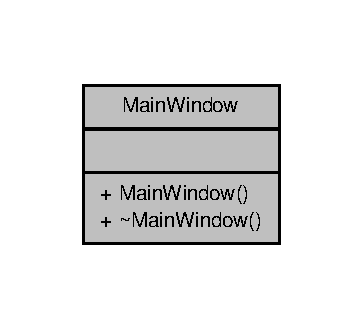
\includegraphics[width=174pt]{class_main_window__coll__graph}
\end{center}
\end{figure}
\subsection*{Fonctions membres publiques}
\begin{DoxyCompactItemize}
\item 
\hyperlink{class_main_window_a8b244be8b7b7db1b08de2a2acb9409db}{Main\-Window} (Q\-Widget $\ast$parent=0)
\begin{DoxyCompactList}\small\item\em \hyperlink{class_main_window_a8b244be8b7b7db1b08de2a2acb9409db}{Main\-Window\-::\-Main\-Window}. \end{DoxyCompactList}\item 
\hyperlink{class_main_window_ae98d00a93bc118200eeef9f9bba1dba7}{$\sim$\-Main\-Window} ()
\end{DoxyCompactItemize}


\subsection{Description détaillée}
on peut retrouver des slots privés et publics qui permettent de quitter le programme et de se connecter 

Définition à la ligne 22 du fichier mainwindow.\-h.



\subsection{Documentation des constructeurs et destructeur}
\hypertarget{class_main_window_a8b244be8b7b7db1b08de2a2acb9409db}{\index{Main\-Window@{Main\-Window}!Main\-Window@{Main\-Window}}
\index{Main\-Window@{Main\-Window}!MainWindow@{Main\-Window}}
\subsubsection[{Main\-Window}]{\setlength{\rightskip}{0pt plus 5cm}Main\-Window\-::\-Main\-Window (
\begin{DoxyParamCaption}
\item[{Q\-Widget $\ast$}]{parent = {\ttfamily 0}}
\end{DoxyParamCaption}
)\hspace{0.3cm}{\ttfamily [explicit]}}}\label{class_main_window_a8b244be8b7b7db1b08de2a2acb9409db}


\hyperlink{class_main_window_a8b244be8b7b7db1b08de2a2acb9409db}{Main\-Window\-::\-Main\-Window}. 


\begin{DoxyParams}{Paramètres}
{\em parent} & \\
\hline
\end{DoxyParams}


Définition à la ligne 28 du fichier mainwindow.\-cpp.


\begin{DoxyCode}
                                      :
    QMainWindow(parent),
    ui(\textcolor{keyword}{new} Ui::MainWindow)
\{
    \textcolor{comment}{//construit un interface}
    ui->setupUi(\textcolor{keyword}{this});
\}
\end{DoxyCode}
\hypertarget{class_main_window_ae98d00a93bc118200eeef9f9bba1dba7}{\index{Main\-Window@{Main\-Window}!$\sim$\-Main\-Window@{$\sim$\-Main\-Window}}
\index{$\sim$\-Main\-Window@{$\sim$\-Main\-Window}!MainWindow@{Main\-Window}}
\subsubsection[{$\sim$\-Main\-Window}]{\setlength{\rightskip}{0pt plus 5cm}Main\-Window\-::$\sim$\-Main\-Window (
\begin{DoxyParamCaption}
{}
\end{DoxyParamCaption}
)}}\label{class_main_window_ae98d00a93bc118200eeef9f9bba1dba7}


Définition à la ligne 36 du fichier mainwindow.\-cpp.


\begin{DoxyCode}
\{
    \textcolor{keyword}{delete} ui;
\}
\end{DoxyCode}


La documentation de cette classe a été générée à partir des fichiers suivants \-:\begin{DoxyCompactItemize}
\item 
/home/afontraille/\-Q\-T C\-R\-E\-A\-T\-O\-R/back\-Office\-N\-W/\hyperlink{mainwindow_8h}{mainwindow.\-h}\item 
/home/afontraille/\-Q\-T C\-R\-E\-A\-T\-O\-R/back\-Office\-N\-W/\hyperlink{mainwindow_8cpp}{mainwindow.\-cpp}\end{DoxyCompactItemize}

\chapter{Documentation des fichiers}
\hypertarget{connexion_8cpp}{\section{Référence du fichier /home/afontraille/\-Q\-T C\-R\-E\-A\-T\-O\-R/back\-Office\-N\-W/connexion.cpp}
\label{connexion_8cpp}\index{/home/afontraille/\-Q\-T C\-R\-E\-A\-T\-O\-R/back\-Office\-N\-W/connexion.\-cpp@{/home/afontraille/\-Q\-T C\-R\-E\-A\-T\-O\-R/back\-Office\-N\-W/connexion.\-cpp}}
}


Permet de pouvoir se connecter ou s'inscrire dans New World.  


{\ttfamily \#include \char`\"{}connexion.\-h\char`\"{}}\\*
{\ttfamily \#include \char`\"{}ui\-\_\-connexion.\-h\char`\"{}}\\*
{\ttfamily \#include \char`\"{}gestion.\-h\char`\"{}}\\*
{\ttfamily \#include $<$Q\-Sql\-Query$>$}\\*
{\ttfamily \#include $<$Q\-Message\-Box$>$}\\*
{\ttfamily \#include $<$Q\-Debug$>$}\\*
Graphe des dépendances par inclusion de connexion.\-cpp\-:\nopagebreak
\begin{figure}[H]
\begin{center}
\leavevmode
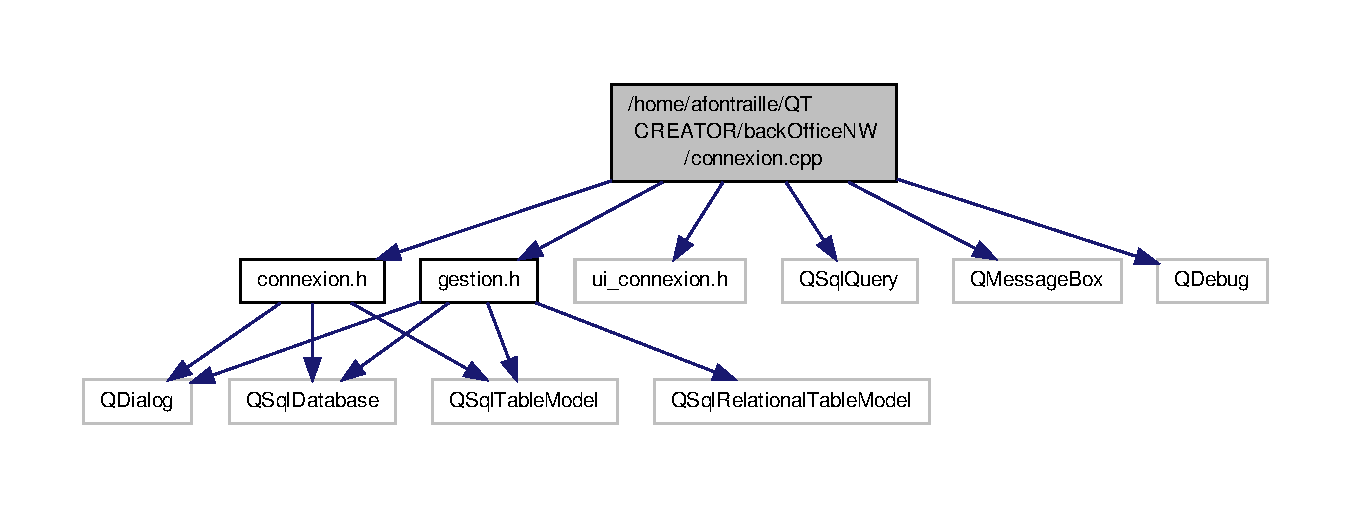
\includegraphics[width=350pt]{connexion_8cpp__incl}
\end{center}
\end{figure}


\subsection{Description détaillée}
Permet de pouvoir se connecter ou s'inscrire dans New World. \begin{DoxyAuthor}{Auteur}
A.\-Fontraille 
\end{DoxyAuthor}
\begin{DoxyRefDesc}{Bogue}
\item[\hyperlink{bug__bug000001}{Bogue}]ne permet pas vraiment de s'inscrire, seulement de se connecter identifiant \-: afontraille mdp \-: 123 \end{DoxyRefDesc}
\begin{DoxyDate}{Date}
4 septembre 2015 
\end{DoxyDate}
\begin{DoxyVersion}{Version}
1 
\end{DoxyVersion}


Définition dans le fichier \hyperlink{connexion_8cpp_source}{connexion.\-cpp}.


\hypertarget{connexion_8h}{\section{Référence du fichier /home/afontraille/\-Q\-T C\-R\-E\-A\-T\-O\-R/back\-Office\-N\-W/connexion.h}
\label{connexion_8h}\index{/home/afontraille/\-Q\-T C\-R\-E\-A\-T\-O\-R/back\-Office\-N\-W/connexion.\-h@{/home/afontraille/\-Q\-T C\-R\-E\-A\-T\-O\-R/back\-Office\-N\-W/connexion.\-h}}
}


Permet de pouvoir se connecter ou s'inscrire dans New World.  


{\ttfamily \#include $<$Q\-Dialog$>$}\\*
{\ttfamily \#include $<$Q\-Sql\-Database$>$}\\*
{\ttfamily \#include $<$Q\-Sql\-Table\-Model$>$}\\*
Graphe des dépendances par inclusion de connexion.\-h\-:\nopagebreak
\begin{figure}[H]
\begin{center}
\leavevmode
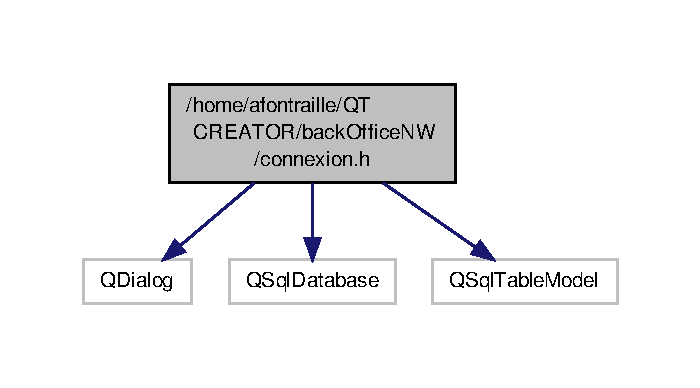
\includegraphics[width=336pt]{connexion_8h__incl}
\end{center}
\end{figure}
Ce graphe montre quels fichiers incluent directement ou indirectement ce fichier \-:\nopagebreak
\begin{figure}[H]
\begin{center}
\leavevmode
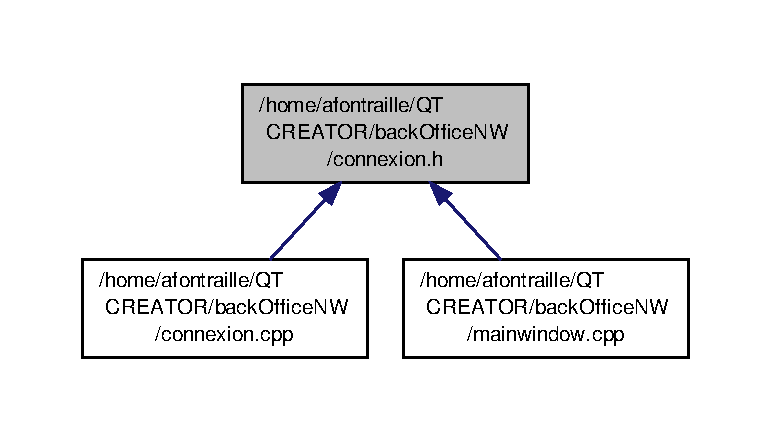
\includegraphics[width=350pt]{connexion_8h__dep__incl}
\end{center}
\end{figure}
\subsection*{Classes}
\begin{DoxyCompactItemize}
\item 
class \hyperlink{classconnexion}{connexion}
\begin{DoxyCompactList}\small\item\em avec la classe connexion on retrouve des slots privés et publics ils permettent de valider ou tout simplement de fermer la fenêtre nous pouvons aussi gérer la couleur \end{DoxyCompactList}\end{DoxyCompactItemize}
\subsection*{Espaces de nommage}
\begin{DoxyCompactItemize}
\item 
namespace \hyperlink{namespace_ui}{Ui}
\end{DoxyCompactItemize}


\subsection{Description détaillée}
Permet de pouvoir se connecter ou s'inscrire dans New World. \begin{DoxyDate}{Date}
4 septembre 2015
\end{DoxyDate}
\begin{DoxyAuthor}{Auteur}
A.\-Fontraille 
\end{DoxyAuthor}
\begin{DoxyVersion}{Version}
1 
\end{DoxyVersion}


Définition dans le fichier \hyperlink{connexion_8h_source}{connexion.\-h}.


\hypertarget{gestion_8cpp}{\section{Référence du fichier /home/afontraille/\-Q\-T C\-R\-E\-A\-T\-O\-R/back\-Office\-N\-W/gestion.cpp}
\label{gestion_8cpp}\index{/home/afontraille/\-Q\-T C\-R\-E\-A\-T\-O\-R/back\-Office\-N\-W/gestion.\-cpp@{/home/afontraille/\-Q\-T C\-R\-E\-A\-T\-O\-R/back\-Office\-N\-W/gestion.\-cpp}}
}


Permet de pouvoir gérer les produits et les rayons.  


{\ttfamily \#include \char`\"{}gestion.\-h\char`\"{}}\\*
{\ttfamily \#include \char`\"{}ui\-\_\-gestion.\-h\char`\"{}}\\*
{\ttfamily \#include $<$Q\-Message\-Box$>$}\\*
{\ttfamily \#include $<$Q\-Sql\-Query$>$}\\*
{\ttfamily \#include $<$Q\-Sql\-Relational\-Table\-Model$>$}\\*
{\ttfamily \#include $<$Q\-Sql\-Relation$>$}\\*
{\ttfamily \#include $<$Q\-Sql\-Table\-Model$>$}\\*
{\ttfamily \#include $<$Q\-Sql\-Relational\-Delegate$>$}\\*
{\ttfamily \#include $<$Q\-Sql\-Record$>$}\\*
{\ttfamily \#include $<$Q\-Model\-Index$>$}\\*
Graphe des dépendances par inclusion de gestion.\-cpp\-:\nopagebreak
\begin{figure}[H]
\begin{center}
\leavevmode
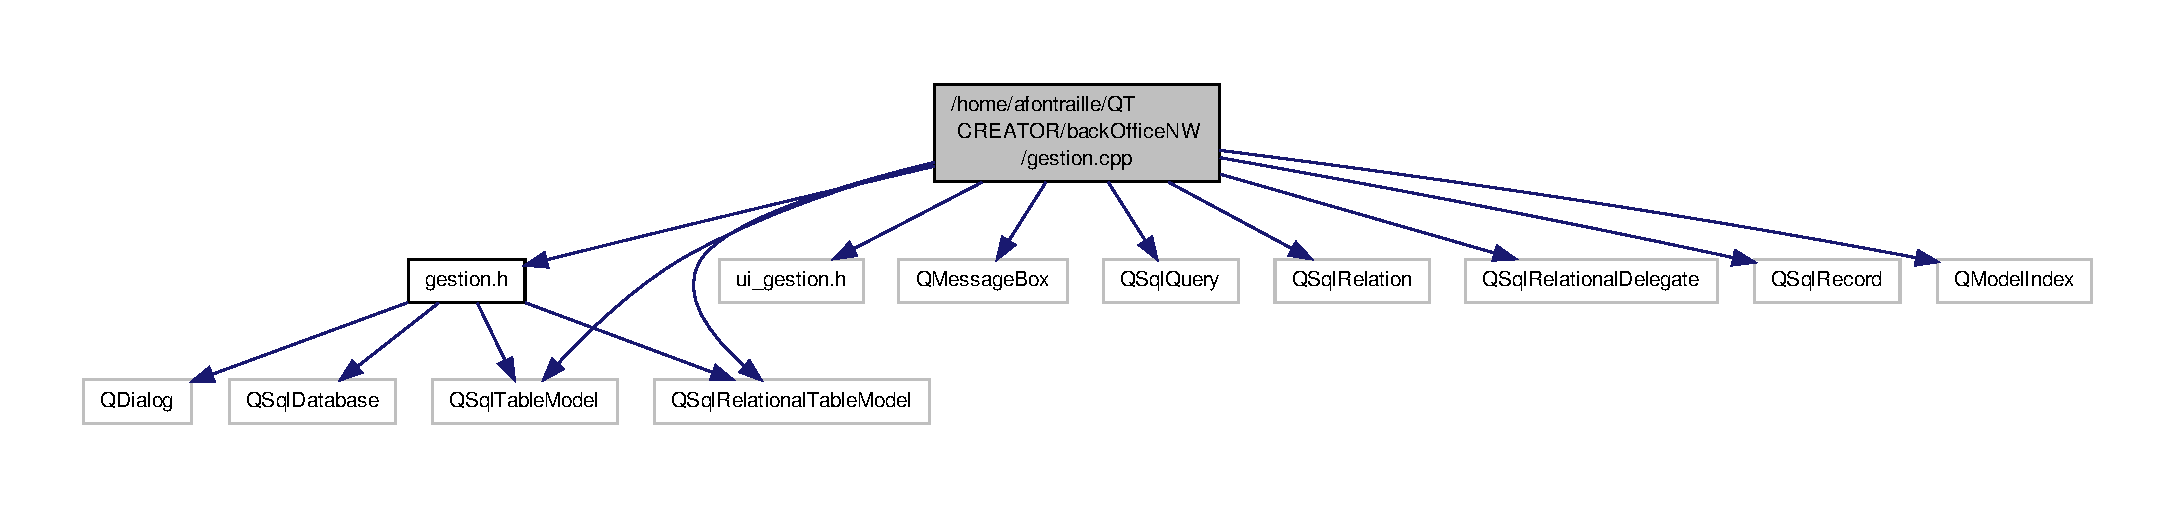
\includegraphics[width=350pt]{gestion_8cpp__incl}
\end{center}
\end{figure}


\subsection{Description détaillée}
Permet de pouvoir gérer les produits et les rayons. \begin{DoxyAuthor}{Auteur}
A.\-Fontraille 
\end{DoxyAuthor}
\begin{DoxyDate}{Date}
4 septembre 2015 
\end{DoxyDate}
\begin{DoxyVersion}{Version}
1 
\end{DoxyVersion}


Définition dans le fichier \hyperlink{gestion_8cpp_source}{gestion.\-cpp}.


\hypertarget{gestion_8h}{\section{Référence du fichier /home/afontraille/\-Q\-T C\-R\-E\-A\-T\-O\-R/back\-Office\-N\-W/gestion.h}
\label{gestion_8h}\index{/home/afontraille/\-Q\-T C\-R\-E\-A\-T\-O\-R/back\-Office\-N\-W/gestion.\-h@{/home/afontraille/\-Q\-T C\-R\-E\-A\-T\-O\-R/back\-Office\-N\-W/gestion.\-h}}
}


permet de pouvoir gérer les produits et les rayons  


{\ttfamily \#include $<$Q\-Dialog$>$}\\*
{\ttfamily \#include $<$Q\-Sql\-Database$>$}\\*
{\ttfamily \#include $<$Q\-Sql\-Table\-Model$>$}\\*
{\ttfamily \#include $<$Q\-Sql\-Relational\-Table\-Model$>$}\\*
Graphe des dépendances par inclusion de gestion.\-h\-:\nopagebreak
\begin{figure}[H]
\begin{center}
\leavevmode
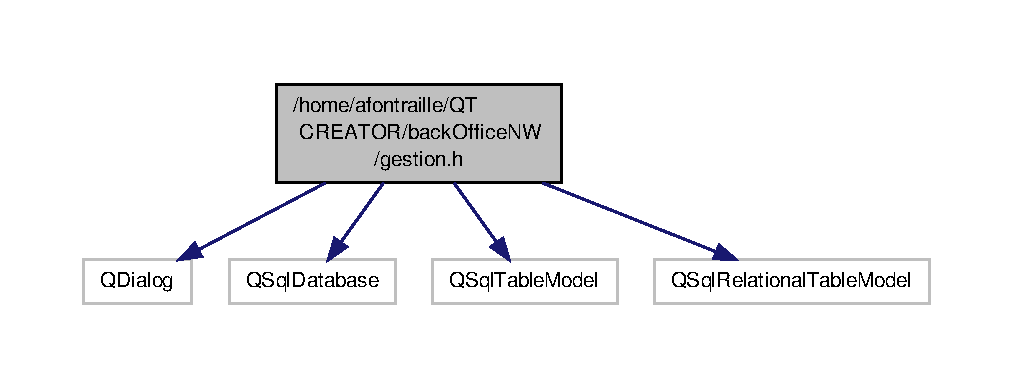
\includegraphics[width=350pt]{gestion_8h__incl}
\end{center}
\end{figure}
Ce graphe montre quels fichiers incluent directement ou indirectement ce fichier \-:\nopagebreak
\begin{figure}[H]
\begin{center}
\leavevmode
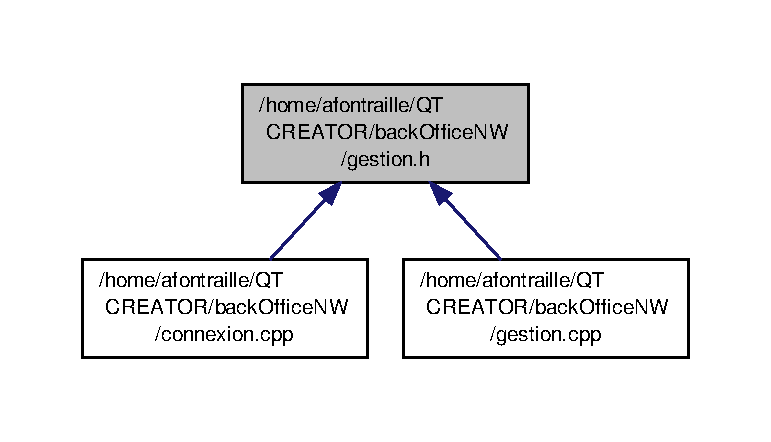
\includegraphics[width=350pt]{gestion_8h__dep__incl}
\end{center}
\end{figure}
\subsection*{Classes}
\begin{DoxyCompactItemize}
\item 
class \hyperlink{classgestion}{gestion}
\begin{DoxyCompactList}\small\item\em Avec la classe gestion on retrouve les slots privés ou public afin de gérer les différents rayons et produits on peut donc supprimer, ajouter ou modifier puis tout simplement les voir on peut également gérer la couleur. \end{DoxyCompactList}\end{DoxyCompactItemize}
\subsection*{Espaces de nommage}
\begin{DoxyCompactItemize}
\item 
namespace \hyperlink{namespace_ui}{Ui}
\end{DoxyCompactItemize}


\subsection{Description détaillée}
permet de pouvoir gérer les produits et les rayons \begin{DoxyDate}{Date}
4 septembre 2015
\end{DoxyDate}
\begin{DoxyAuthor}{Auteur}
A.\-Fontraille 
\end{DoxyAuthor}
\begin{DoxyVersion}{Version}
1 
\end{DoxyVersion}


Définition dans le fichier \hyperlink{gestion_8h_source}{gestion.\-h}.


\hypertarget{main_8cpp}{\section{Référence du fichier /home/afontraille/\-Q\-T C\-R\-E\-A\-T\-O\-R/back\-Office\-N\-W/main.cpp}
\label{main_8cpp}\index{/home/afontraille/\-Q\-T C\-R\-E\-A\-T\-O\-R/back\-Office\-N\-W/main.\-cpp@{/home/afontraille/\-Q\-T C\-R\-E\-A\-T\-O\-R/back\-Office\-N\-W/main.\-cpp}}
}


main est obligatoire dans tout les programmes c++  


{\ttfamily \#include $<$Q\-Application$>$}\\*
{\ttfamily \#include \char`\"{}mainwindow.\-h\char`\"{}}\\*
Graphe des dépendances par inclusion de main.\-cpp\-:\nopagebreak
\begin{figure}[H]
\begin{center}
\leavevmode
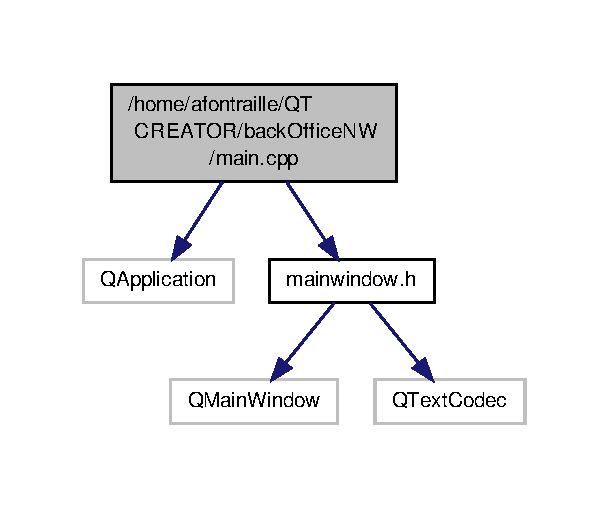
\includegraphics[width=292pt]{main_8cpp__incl}
\end{center}
\end{figure}
\subsection*{Fonctions}
\begin{DoxyCompactItemize}
\item 
int \hyperlink{main_8cpp_a0ddf1224851353fc92bfbff6f499fa97}{main} (int argc, char $\ast$argv\mbox{[}$\,$\mbox{]})
\begin{DoxyCompactList}\small\item\em permet de gérer toutes les fonctionnalités avec main main est obligatoire dans tout les programmes c++ \end{DoxyCompactList}\end{DoxyCompactItemize}


\subsection{Description détaillée}
main est obligatoire dans tout les programmes c++ \begin{DoxyAuthor}{Auteur}
A.\-Fontraille 
\end{DoxyAuthor}
\begin{DoxyDate}{Date}
4 septembre 2015 
\end{DoxyDate}
\begin{DoxyVersion}{Version}
1 
\end{DoxyVersion}


Définition dans le fichier \hyperlink{main_8cpp_source}{main.\-cpp}.



\subsection{Documentation des fonctions}
\hypertarget{main_8cpp_a0ddf1224851353fc92bfbff6f499fa97}{\index{main.\-cpp@{main.\-cpp}!main@{main}}
\index{main@{main}!main.cpp@{main.\-cpp}}
\subsubsection[{main}]{\setlength{\rightskip}{0pt plus 5cm}int main (
\begin{DoxyParamCaption}
\item[{int}]{argc, }
\item[{char $\ast$}]{argv\mbox{[}$\,$\mbox{]}}
\end{DoxyParamCaption}
)}}\label{main_8cpp_a0ddf1224851353fc92bfbff6f499fa97}


permet de gérer toutes les fonctionnalités avec main main est obligatoire dans tout les programmes c++ 


\begin{DoxyParams}{Paramètres}
{\em argc} & \\
\hline
{\em argv} & \\
\hline
\end{DoxyParams}
\begin{DoxyReturn}{Renvoie}

\end{DoxyReturn}


Définition à la ligne 20 du fichier main.\-cpp.


\begin{DoxyCode}
\{
    QApplication a(argc, argv);
    \hyperlink{class_main_window}{MainWindow} w;
    w.show();
    
    \textcolor{keywordflow}{return} a.exec();
    QTextCodec::setCodecForTr(QTextCodec::codecForName(\textcolor{stringliteral}{"UTF-8"}));
    QTextCodec::setCodecForLocale(QTextCodec::codecForName(\textcolor{stringliteral}{"UTF-8"}));
    QTextCodec::setCodecForCStrings(QTextCodec::codecForName(\textcolor{stringliteral}{"UTF-8"}));
    \textcolor{comment}{//modelProduit->setHeaderData(0, Qt::Horizontal, trUtf8("Identifiant"));}
\}
\end{DoxyCode}

\hypertarget{mainwindow_8cpp}{\section{Référence du fichier /home/afontraille/\-Q\-T C\-R\-E\-A\-T\-O\-R/back\-Office\-N\-W/mainwindow.cpp}
\label{mainwindow_8cpp}\index{/home/afontraille/\-Q\-T C\-R\-E\-A\-T\-O\-R/back\-Office\-N\-W/mainwindow.\-cpp@{/home/afontraille/\-Q\-T C\-R\-E\-A\-T\-O\-R/back\-Office\-N\-W/mainwindow.\-cpp}}
}
{\ttfamily \#include \char`\"{}mainwindow.\-h\char`\"{}}\\*
{\ttfamily \#include \char`\"{}ui\-\_\-mainwindow.\-h\char`\"{}}\\*
{\ttfamily \#include \char`\"{}connexion.\-h\char`\"{}}\\*
{\ttfamily \#include $<$Q\-Message\-Box$>$}\\*
{\ttfamily \#include $<$Q\-Sql\-Record$>$}\\*
{\ttfamily \#include $<$Q\-Text\-Codec$>$}\\*
{\ttfamily \#include $<$Q\-String$>$}\\*
{\ttfamily \#include $<$Q\-Debug$>$}\\*
{\ttfamily \#include $<$Q\-Palette$>$}\\*
{\ttfamily \#include $<$Q\-Color$>$}\\*
{\ttfamily \#include $<$Q\-Color\-Dialog$>$}\\*
{\ttfamily \#include $<$Q\-Dialog$>$}\\*
{\ttfamily \#include $<$Q\-Sql\-Query$>$}\\*
{\ttfamily \#include $<$Q\-Object$>$}\\*
Graphe des dépendances par inclusion de mainwindow.\-cpp\-:\nopagebreak
\begin{figure}[H]
\begin{center}
\leavevmode
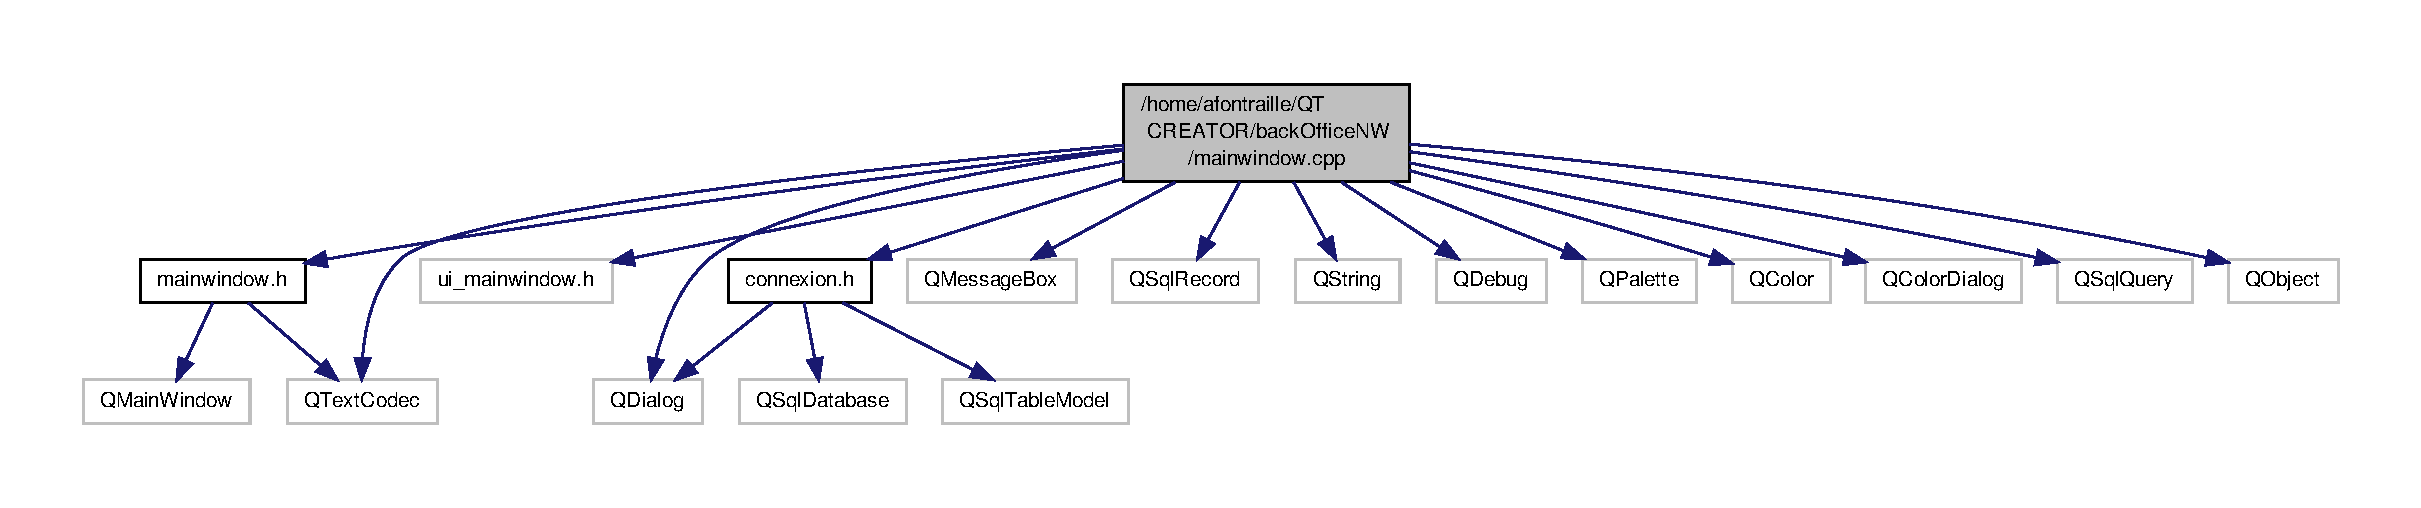
\includegraphics[width=350pt]{mainwindow_8cpp__incl}
\end{center}
\end{figure}


\subsection{Description détaillée}
\begin{DoxyAuthor}{Auteur}
A.\-Fontraille 
\end{DoxyAuthor}
\begin{DoxyDate}{Date}
4 septembre 2015 
\end{DoxyDate}
\begin{DoxyVersion}{Version}
1 
\end{DoxyVersion}


Définition dans le fichier \hyperlink{mainwindow_8cpp_source}{mainwindow.\-cpp}.


\hypertarget{mainwindow_8h}{\section{Référence du fichier /home/afontraille/\-Q\-T C\-R\-E\-A\-T\-O\-R/back\-Office\-N\-W/mainwindow.h}
\label{mainwindow_8h}\index{/home/afontraille/\-Q\-T C\-R\-E\-A\-T\-O\-R/back\-Office\-N\-W/mainwindow.\-h@{/home/afontraille/\-Q\-T C\-R\-E\-A\-T\-O\-R/back\-Office\-N\-W/mainwindow.\-h}}
}
{\ttfamily \#include $<$Q\-Main\-Window$>$}\\*
{\ttfamily \#include $<$Q\-Text\-Codec$>$}\\*
Graphe des dépendances par inclusion de mainwindow.\-h\-:\nopagebreak
\begin{figure}[H]
\begin{center}
\leavevmode
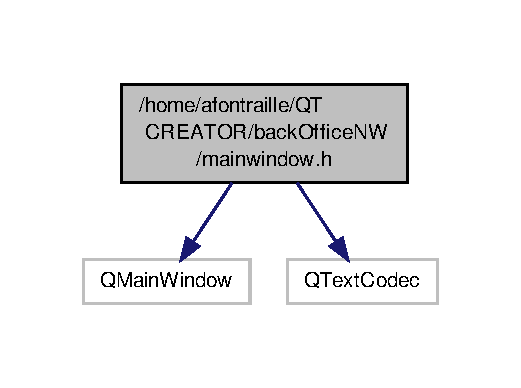
\includegraphics[width=250pt]{mainwindow_8h__incl}
\end{center}
\end{figure}
Ce graphe montre quels fichiers incluent directement ou indirectement ce fichier \-:\nopagebreak
\begin{figure}[H]
\begin{center}
\leavevmode
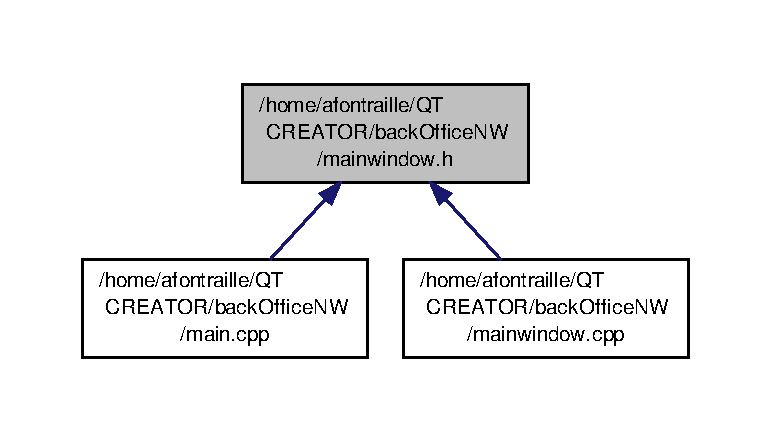
\includegraphics[width=350pt]{mainwindow_8h__dep__incl}
\end{center}
\end{figure}
\subsection*{Classes}
\begin{DoxyCompactItemize}
\item 
class \hyperlink{class_main_window}{Main\-Window}
\begin{DoxyCompactList}\small\item\em on peut retrouver des slots privés et publics qui permettent de quitter le programme et de se connecter \end{DoxyCompactList}\end{DoxyCompactItemize}
\subsection*{Espaces de nommage}
\begin{DoxyCompactItemize}
\item 
namespace \hyperlink{namespace_ui}{Ui}
\end{DoxyCompactItemize}


\subsection{Description détaillée}
\begin{DoxyDate}{Date}
4 septembre 2015 
\end{DoxyDate}
\begin{DoxyVersion}{Version}
1 
\end{DoxyVersion}


Définition dans le fichier \hyperlink{mainwindow_8h_source}{mainwindow.\-h}.


\printindex
\end{document}
